% !TEX TS-program = lualatex
% !TEX encoding = UTF-8 Unicode		

\documentclass[12pt, letterpaper]{article}

%%BIBLIOGRAPHY- This uses biber/biblatex to generate bibliographies according to the 
%%Unified Style Sheet for Linguistics
\usepackage[main=american, german]{babel}% Recommended
\usepackage{csquotes}% Recommended
\usepackage[backend=biber,
		style=unified,
		maxcitenames=3,
		maxbibnames=99,
		natbib,
		url=false]{biblatex}
\addbibresource{../Library.bib}
\setcounter{biburlnumpenalty}{100}  % allow URL breaks at numbers
%\setcounter{biburlucpenalty}{100}   % allow URL breaks at uppercase letters
%\setcounter{biburllcpenalty}{100}   % allow URL breaks at lowercase letters

%%TYPOLOGY
\usepackage[svgnames]{xcolor} % Specify colors by their 'svgnames', for a full list of all colors available see here: http://www.latextemplates.com/svgnames-colors
%\usepackage[compact]{titlesec}
%\titleformat{\section}[runin]{\normalfont\bfseries}{\thesection.}{.5em}{}[.]
%\titleformat{\subsection}[runin]{\normalfont\scshape}{\thesubsection}{.5em}{}[.]
\usepackage[hmargin=1in,vmargin=1in]{geometry}  %Margins          
\usepackage{graphicx}	%Inserting graphics, pictures, images 		
\usepackage{stackengine} %Package to allow text above or below other text, Also helpful for HG weights 
\usepackage{fontspec} %Selection of fonts must be ran in XeLaTeX or LuaLaTeX
\usepackage{amssymb} %Math symbols
\usepackage{amsmath} % Mathematical enhancements for LaTeX
\usepackage{setspace} %Linespacing
\usepackage{multicol} %Multicolumn text
\usepackage{enumitem} %Allows for continuous numbering of lists over examples, etc.
\usepackage{multirow} %Useful for combining cells in tablesbrew 
\usepackage{booktabs}
\usepackage{hanging}
\usepackage{fancyhdr} %Allows for the 
\pagestyle{fancy}
\fancyhead[L]{\textit{QP Handout}} 
\fancyhead[R]{\textit{\today}} 
\fancyfoot[L,R]{} 
\fancyfoot[C]{\thepage} 
\renewcommand{\headrulewidth}{0.4pt}
\setlength{\headheight}{14.5pt} % ...at least 14.49998pt
% \usepackage{fourier} % This allows for the use of certain wingdings like bombs, frowns, etc.
% \usepackage{fourier-orns} %More useful symbols like bombs and jolly-roger, mostly for OT
\usepackage[colorlinks,allcolors={black},urlcolor={blue}]{hyperref} %allows for hyperlinks and pdf bookmarks
% \usepackage{url} %allows for urls
% \def\UrlBreaks{\do\/\do-} %allows for urls to be broken up
\usepackage[normalem]{ulem} %strike out text. Handy for syntax
\usepackage{tcolorbox}
\usepackage{datetime2}

%%FONTS
\setmainfont{Libertinus Serif}
\setsansfont{Libertinus Sans}
\setmonofont[Scale=MatchLowercase]{Libertinus Mono}

%%PACKAGES FOR LINGUISTICS
%\usepackage{OTtablx} %Generating tableaux with using TIPA
\usepackage[noipa]{OTtablx} % Use this one generating tableaux without using TIPA
%\usepackage[notipa]{ot-tableau} % Another tableau drawing packing use for posters.
% \usepackage{linguex} % Linguistic examples
% \usepackage{langsci-linguex} % Linguistic examples
\usepackage{langsci-gb4e} % Language Science Press' modification of gb4e
% \usepackage{langsci-avm} % Language Science Press' AVM package
\usepackage{tikz} % Drawing Hasse diagrams
% \usepackage{pst-asr} % Drawing autosegmental features
\usepackage{pstricks} % required for pst-asr, OTtablx, pst-jtree.
% \usepackage{pst-jtree} 	% Syntax tree draawing software
% \usepackage{tikz-qtree}	% Another syntax tree drawing software. Uses bracket notation.
\usepackage[linguistics]{forest}	% Another syntax tree drawing software. Uses bracket notation.
% \usepackage{ling-macros} % Various linguistic macros. Does not work with linguex.
% \usepackage{covington} % Another linguistic examples package.
\usepackage{leipzig} %	Offers support for Leipzig Glossing Rules

%%LEIPZIG GLOSSING FOR ZAPOTEC
\newleipzig{el}{el}{elder}	% Elder pronouns
\newleipzig{hu}{hu}{human}	% Human pronouns
\newleipzig{an}{an}{animate}	% Animate pronouns
\newleipzig{in}{in}{inanimate}	% Inanimate pronouns
\newleipzig{pot}{pot}{potential}	% Potential Aspect
\newleipzig{cont}{cont}{continuative}	% Continuative Aspect
% \newleipzig{pot}{pot}{potential}	% Potential Aspect
\newleipzig{stat}{stat}{stative}	% Potential Aspect
\newleipzig{and}{and}{andative}	% Andative Aspect
\newleipzig{ven}{ven}{venative}	% Venative Aspect
% \newleipzig{res}{res}{restitutive}	% Restitutive Aspect
\newleipzig{rep}{rep}{repetitive}	% Repetitive Aspect

%%TITLE INFORMATION
\title{TITLE}
\author{Mykel Loren Brinkerhoff}
\date{\today}

%%MACROS
\newcommand{\sub}[1]{\textsubscript{#1}}
\newcommand{\supr}[1]{\textsuperscript{#1}}
\providecommand{\lsptoprule}{\midrule\toprule}
\providecommand{\lspbottomrule}{\bottomrule\midrule}
\newcommand{\fittable}[1]{\resizebox{\textwidth}{!}{#1}}

\makeatletter
\renewcommand{\paragraph}{%
  \@startsection{paragraph}{4}%
  {\z@}{0ex \@plus 1ex \@minus .2ex}{-1em}%
  {\normalfont\normalsize\bfseries}%
}
\makeatother
\parindent=10pt


\begin{document}
	
%%If using linguex, need the following commands to get correct LSA style spacing
%% these have to be after  \begin{document}
	% \setlength{\Extopsep}{6pt}
	% \setlength{\Exlabelsep}{9pt}		%effect of 0.4in indent from left text edge
%%
	
%% Line spacing setting. Comment out the line spacing you do not need. Comment out all if you want single spacing.
%	\doublespacing
%	\onehalfspacing
	
\begin{center}
	{\Large \textbf{Investigating the timing of tone and phonation in Santiago Laxopa Zapotec. }}
	\vspace{6pt}

	Mykel Loren Brinkerhoff
\end{center}
%\maketitle
%\maketitleinst
\thispagestyle{fancy}

\tableofcontents


%------------------------------------
\section{Introduction} \label{sec:Introduction}
%------------------------------------

\begin{itemize}
	\item Most work on the interaction of tone and phonation has been based on descriptions of southeast and far east Asian languages.
	\item This lead to strong claims on the interaction between tone and phonation \citep{masicaDefiningLinguisticArea1976,thurgoodVietnameseTonogenesisRevising2002,yipTone2002,enfieldArealLinguisticsMainland2005,michaudComplexTonesEast2012,brunelleTonePhonationSoutheast2016}.
	\item Main claim from these authors is that tone and phonation are codependent. This is often referred to as a register system.  
	\begin{itemize}
		\item Meaning that we only observe certain tones with certain phonations. 
		\item Mandarin Tone 3 is always associated with creaky voice \citep{duanmuPhonologyStandardChinese2007}.
	\end{itemize}
	\item This claim has also been made in the reverse that certain phonation types are associated with specific tonal patterns. 
	\begin{itemize}
		\item Breathy voice stereotypically appears with high pitch and creaky voice sterotypically appears with low pitch \citep{eslingVoiceQualityLaryngeal2019}.
		\begin{itemize}
			\item TODO:\/\/ Look for earlier references to these claims. 
		\end{itemize}
		\item This is often born out with research into register systems. 
		\item Also found in pathological voice quality \citep{klattAnalysisSynthesisPerception1990,titzePrinciplesVoiceProduction2000,eslingVoiceQualityLaryngeal2019}.
	\end{itemize}
	\item Research into Mesoamerican languages, however, shows that these claims are too strong or exaggerated \citep{suarezMesoamericanIndianLanguages1983,campbellMesoAmericaLinguisticArea1986,silvermanLaryngealComplexityOtomanguean1997,dicanioPhoneticsPhonologySan2008,espositoVariationContrastivePhonation2010, campbellOtomangueanHistoricalLinguistics2017a,campbellOtomangueanHistoricalLinguistics2017}. 
	\item Most languages of the Oto-Manguean language family exhibits independent tone and phonation.
	\begin{itemize}
		\item Tone and phonation freely co-occur or exhibit a much freer distribution than what is found in register languages. 
		\item San Lucas Quiaviní Zapotec is one such example.
	\end{itemize}
\end{itemize}

\begin{table}[!ht]
	\centering
	\caption{SLQZ tone and phonation}
	\label{tab:SLQZ}
	\begin{tabular}{lcccc}
		\lsptoprule
						&	 Modal  & Breathy & Creaky & Interrupted \\
			High	& ✔︎ & -- & ✔︎ & ✔︎ \\
			Low & ✔︎ & ✔︎ & ✔︎ & ✔︎ \\
			Falling & ✔︎ & ✔︎ & ✔︎ & ✔︎ \\
			Rising & ✔︎ & -- & -- & -- \\
		\lspbottomrule
	\end{tabular}
\end{table}
\begin{itemize}
	\item This paper adds to this debate by:
	\begin{itemize}
		\item Providing another description of a language that uses tone and phonation
		\item Evaluates the claims of \citet{silvermanLaryngealComplexityOtomanguean1997}
	\end{itemize}
\end{itemize}

%------------------------------------
\section{The Laryngeal Complexity Hypothesis} \label{sec:Silverman}
%------------------------------------



%------------------------------------
\section{Santiago Laxopa Zapotec} \label{sec:SLZ}
%------------------------------------

Santiago Laxopa Zapotec (SLZ; Dilla'xhonh Laxup) is a Northern Zapotec language spoken by approximately 1000 people in the municipality of Santiago Laxopa, Ixtlán District in the Sierra Norte of Oaxaca, Mexico \citep{adlerAcousticsPhonationTypes2016,adlerDerivationVerbInitiality2018,foleyForbiddenCliticClusters2018,foleyExtendingPersonCaseConstraint2020}. As is common among Zapotecan languages, SLZ distinguishes between lenis and fortis consonants \citep[e.g.,][]{nellisFortisLenisCajonos1980,jaegerFortisLenisQuestion1983,uchiharaFortisLenisGlides2016} and has a fairly standard five-vowel inventory. These contrasts and inventories can be seen in Table~\ref{tab:SLZcons} and Table~\ref{tab:SLZvowels}.


\begin{table}[!h]
	\centering
	\caption{Consonant inventory for Santiago Laxopa Zapotec}
	\label{tab:SLZcons}
	\fittable{
	 \begin{tabular}{llcccccccc}
	  \lsptoprule
		  &  & bilabial & alveolar  & retroflex & alveo- & palatal &velar &labio-  &  uvular \\
		 &&&&& palatal &&&velar& \\
	  \midrule
		nasal    	& lenis   &	   & n  & & & & & & \\
					& fortis  &	mː & nː & & & & & & \\
		stop 		& lenis   & b  & d  & & & & g & gʷ & \\
					   & fortis  & p  & t  & & & & k & kʷ & \\
		fricative   & lenis   &    & z  & ʐ\textasciitilde ɽ & ʒ & ç & &  & ʁ\textasciitilde χ \\
					   & fortis  &    & s  & ʂ & ʃ & & & & \\
		  affricate 	& lenis   &    & d͡z & & & & & & \\
					  & fortis  &    & t͡s & & t͡ʃ & & & & \\
		lateral  	& lenis   &    & l\textasciitilde ɾ & & & & & & \\
					& fortis  &    & lː & & & & & & \\
		trill		& 		  &    & r & & &  & &  & \\ 			
		approximate & 		  &    & & & & j & & w & \\ 
	  \lspbottomrule
	 \end{tabular}
	 }
	\end{table}

	\begin{table}[!h]
		\centering
		\caption{Vowels inventory in Santiago Laxopa Zapotec.}
		\label{tab:SLZvowels}
		 \begin{tabular}{lccc}
		  \lsptoprule
					&  front& central  & back \\
		  \midrule
			high   	&  i  &     &   u \\
			mid    	&  e  &   	& 	o \\
			low   	&     &  a 	&	  \\
		  \lspbottomrule
		 \end{tabular}
		\end{table}
		
In addition to the contrasts in both consonants and vowels, SLZ additionally has a phonation and tonal contrast. I will first talk about the phonation contrasts in Section~\ref{sec:Phonation} followed by the tonal contrasts in Section~\ref{sec:Tone}.

%------------------------------------
\subsection{Phonation in SLZ} \label{sec:Phonation}
%------------------------------------

Among Zapotecan languages it is quite common for languages to make use of contrastive phonation \citep[e.g.,][]{avelinobecerraTopicsYalalagZapotec2004,longDiccionarioZapotecoSan2005,avelinoAcousticElectroglottographicAnalyses2010,lopeznicolasEstudiosFonologiaGramatica2016,chavez-peonInteractionMetricalStructure2010}. 
SLZ, in addition to the five vowel qualities, has four contrastive phonation types which are: modal, breathy, checked, and laryngealized. These contrasts are exemplified in the minimal quadruple in (\ref{ex:YA}). 

\ea \label{ex:YA} Four-way minimal phonation contrast
	\ea \textit{ya} [ja\supr{L}]	`bell'
	\ex \textit{yah}  [ja̤\supr{L}] `metal/rifle'
	\ex \textit{ya'}  [jaˀ\supr{L}]  `pound'
	\ex \textit{ya'a}  [jaˀa\supr{L}]  `market'
	\z 
\z 

Breathy phonation on vowels is characterized by a raspy quality throughout the whole vowel or a portion toward the end of the vowel, see Figure~\ref{fig:BreathyVowel}. 

\begin{figure}[!h]
	\centering
	% [INSERT YAH SPECTROGRAM AND WAVEFORM]
	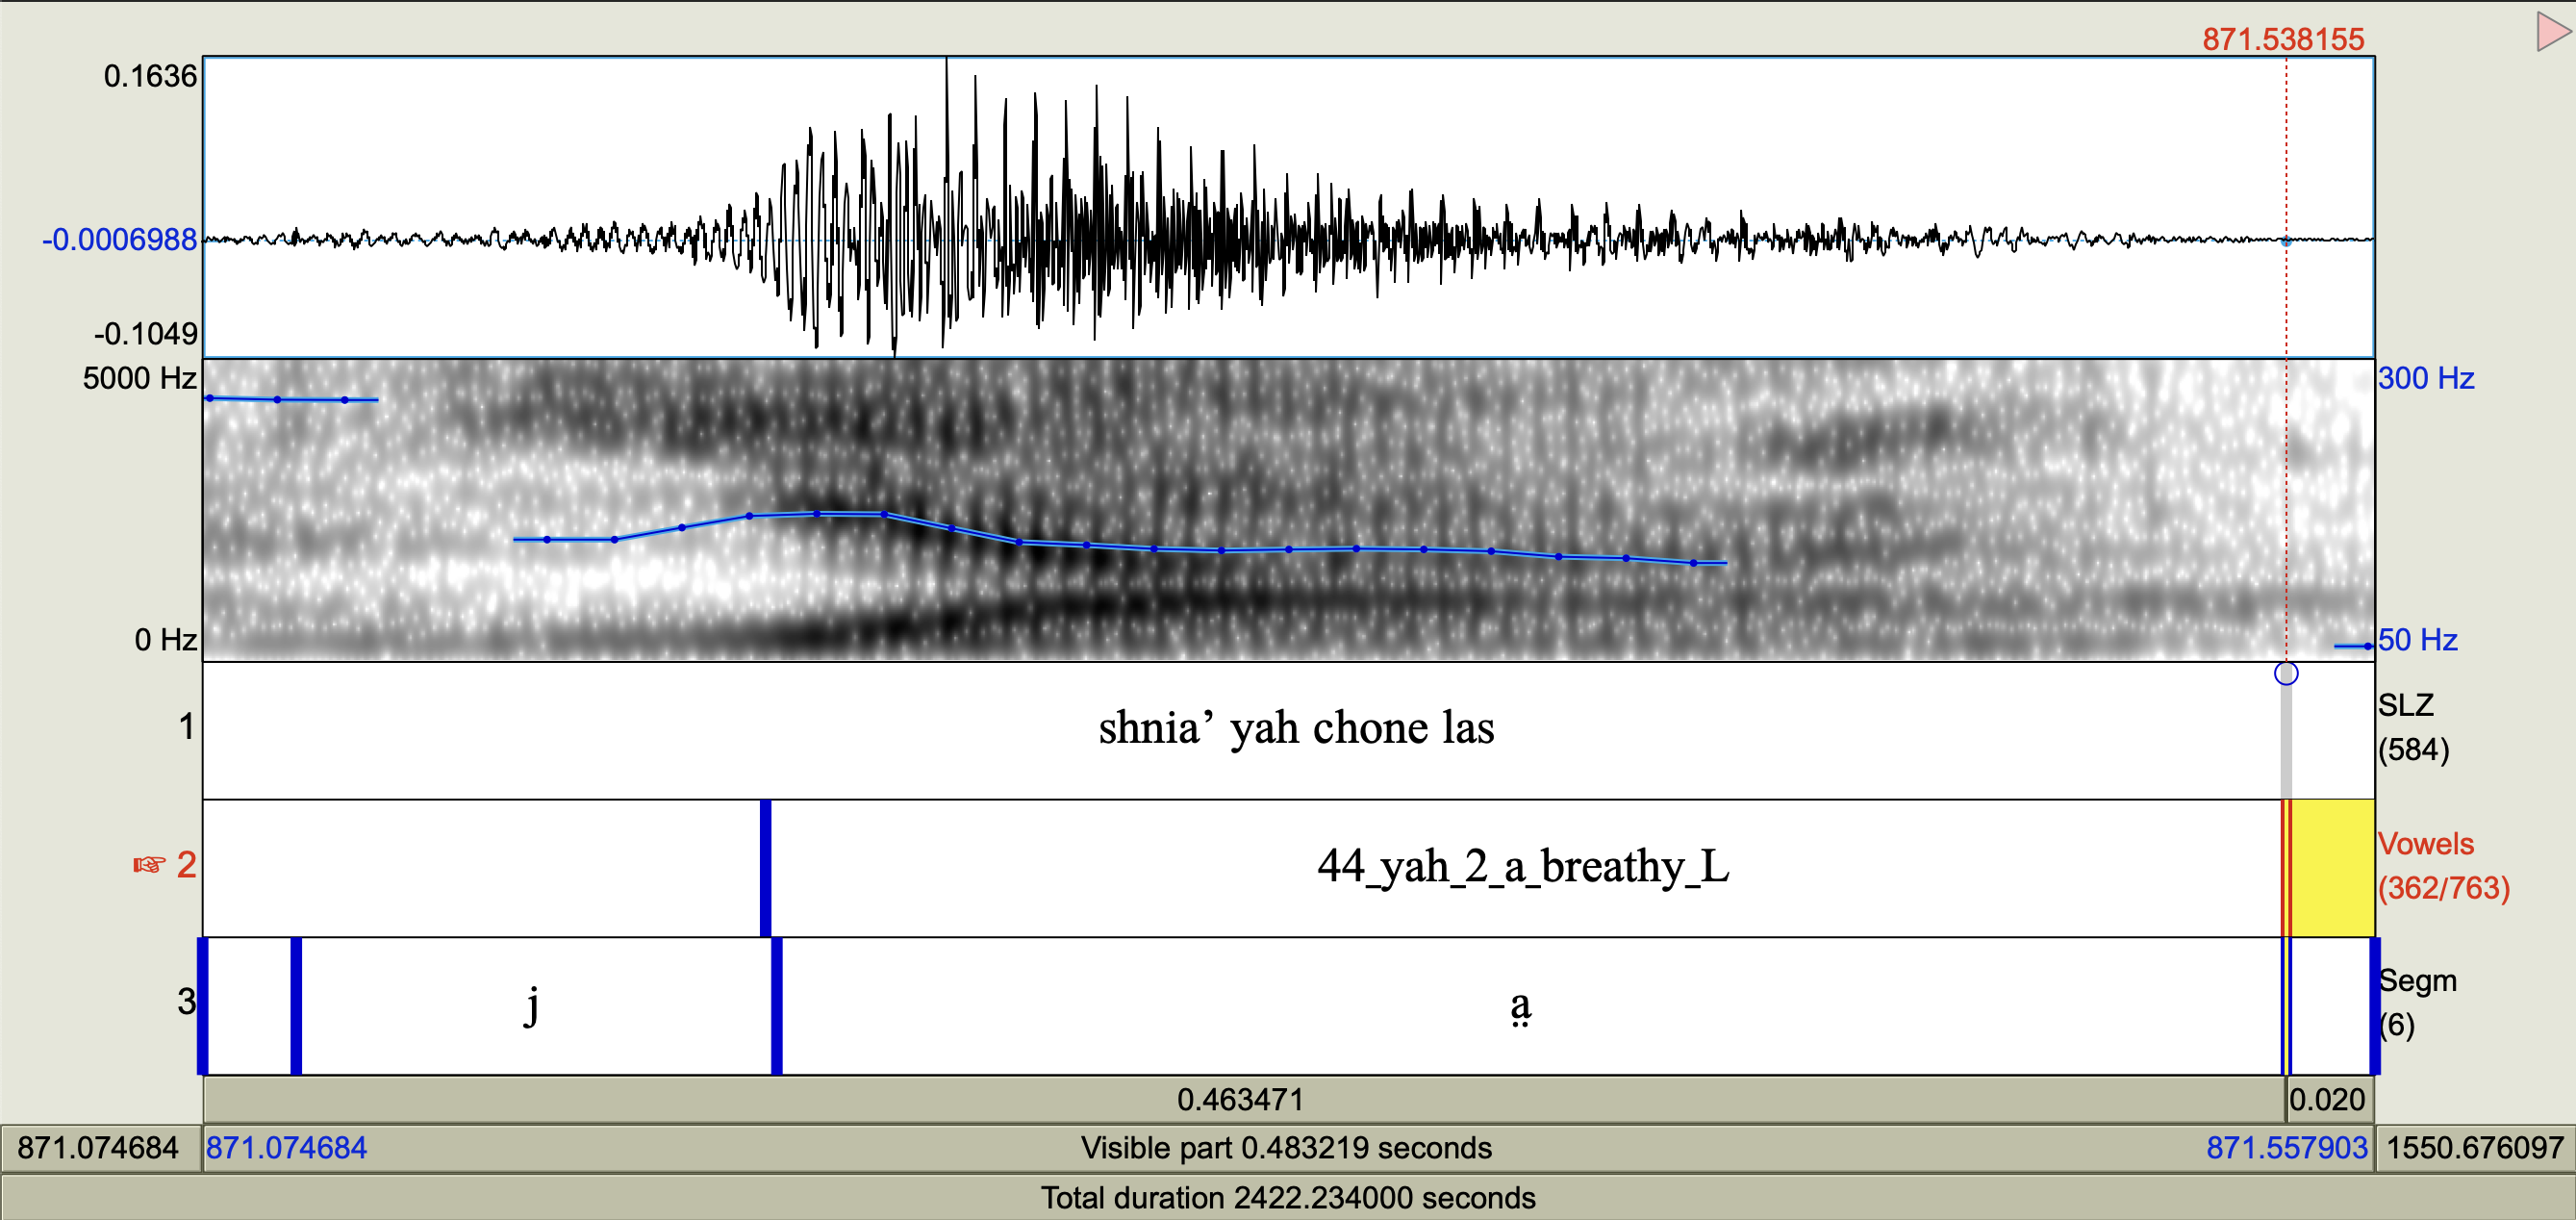
\includegraphics[width=0.9\textwidth]{../yah.png}
	\label{fig:BreathyVowel}
	\caption{Breathy vowel in the word \textit{yah} `metal/rifle'}
\end{figure}

Checked vowels on the other hand are characterized by an abrupt glottal closure which cuts the vowel short. This phonation is sometimes only realized as a very short period of creakiness at the end of the vowel, see Figure~\ref{fig:CheckedVowel}.  

\begin{figure}[!h]
	\centering
	[INSERT YA' SPECTROGRAM AND WAVEFORM]
	% 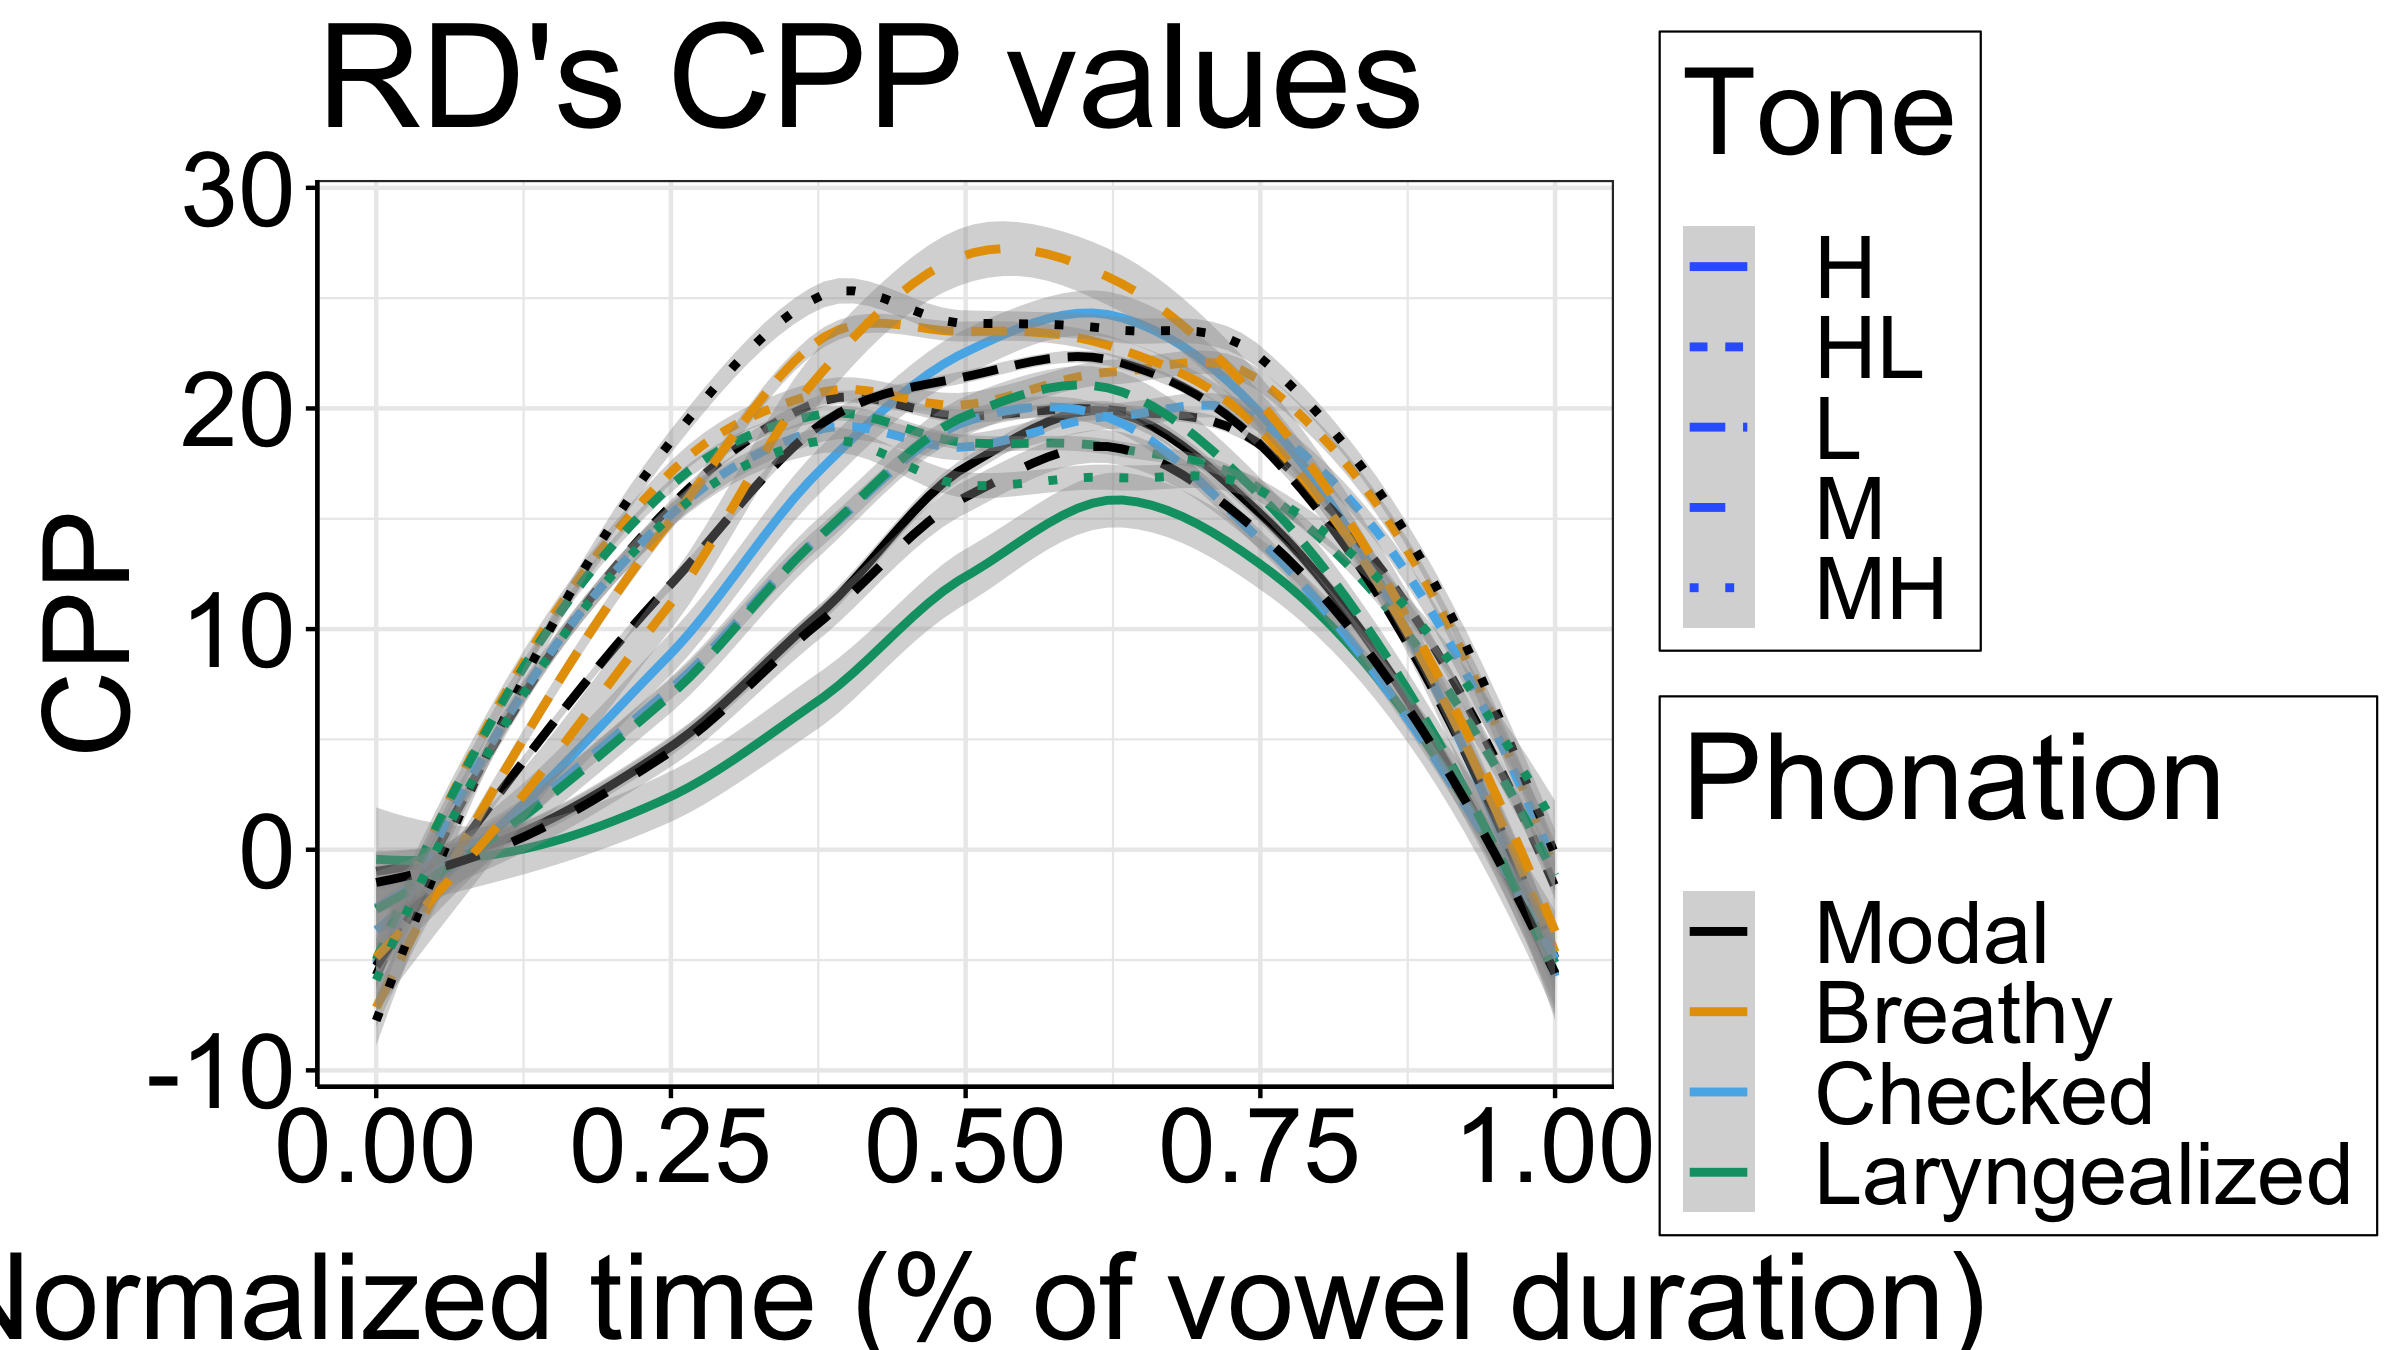
\includegraphics[width=0.9\textwidth]{../RDCPP_line.png}
	\label{fig:CheckedVowel}
	\caption{Breathy vowel in the word \textit{ya'} `pound'}
\end{figure}

Laryngealized vowels are quite common in Zapotecan languages and have received a wide number of different names. Previous descriptions have used terms such as broken, rearticulated, interrupted, and creaky \citep{longDiccionarioZapotecoSan2005,avelinobecerraTopicsYalalagZapotec2004,avelinoAcousticElectroglottographicAnalyses2010,sonnenscheinDescriptiveGrammarSan2005,adlerAcousticsPhonationTypes2016}. In order to avoid confusion, I will use the term laryngealized following \citet{avelinoAcousticElectroglottographicAnalyses2010}. In addition to a wide number of different names these vowels also exhibit a wide range of allophones. 

\citet{avelinoAcousticElectroglottographicAnalyses2010} found in the closely realted Yalálag Zapotec that among his consultants there were at least four different pronunciations as seen in Table~\ref{tab:laryngeal}
\begin{table}[!h]
	\centering
	\caption{Layngealized Vowels in Yalálag Zapotec}
	\label{tab:laryngeal}
	 \begin{tabular}{ll}
	\lsptoprule
	/VˀV/	&  [VʔV]  \\
			&  [VV̰V]   \\
			&  [VV̰ːV̆]  \\
			&  [VV̰V̰]	\\
	\lspbottomrule
	\end{tabular}
\end{table}
In SLZ, each of the consulted language experts would produce this vowel differently. One consultant would do rearticulation, where there is a full glottal stop in the middle of the vowel, or creaky voice. This alternation seemed to be in free variation but there was a greater tendency to creak in low toned words, such as \textit{xa'ag} [ʂa̰ːg] `topil'\footnote{A topil is a type of government office in traditional Oaxacan communities somewhat akin to a sherif. }, see Figure~\ref{fig:FSRLaryngeal} for a comparison between this consultant's pronunciation of the laryngealized vowels.

\begin{figure}[!h]
	\centering
	[INSERT SIDE BY SIDE SPECTROGRAMS]
	\caption{Comparison of FSR's laryngealized vowels in \textit{ya'a} `mountain' and \textit{xa'ag} `topil'}
	\label{fig:FSRLaryngeal}
\end{figure}

The other consultant only ever produces creaky voice for these vowels regardless of the tone with the word. During one of the elicitation sessions, we conducted a sanity check that these were in fact the same vowels and both consultants reliably identified the words and would produce the laryngealized vowel according to their own idiosyncrasies. However, a more detailed perception study is beyond the scope of this paper. 
\begin{figure}[!h]
	\centering
	[INSERT SIDE BY SIDE SPECTROGRAMS]
	\caption{Comparison of RD's laryngealized vowels in \textit{ya'a} `mountain' and \textit{xa'ag} `topil'}
	\label{fig:RDLaryngeal}
\end{figure}

%------------------------------------
\subsection{Tone in SLZ} \label{sec:Tone}
%------------------------------------

As is common among Oto-Manguean languages, SLZ is a tonal languages \citep{suarezMesoamericanIndianLanguages1983,campbellMesoAmericaLinguisticArea1986,silvermanLaryngealComplexityOtomanguean1997,campbellOtomangueanHistoricalLinguistics2017a,campbellOtomangueanHistoricalLinguistics2017}. In SLZ there are five surface tones which appear on a syllable. 


\begin{table}[!h]
	\centering
	\caption{SLZ tones}
	\label{tab:tones}
	 \begin{tabular}{lllll}
	  \lsptoprule
					  % &	 Diacritic  & Example & Transcription \\
	  High   	&  a\supr{H}  &  \textit{xha}   &  [ ʐa\supr{H} ] & `clothing.\textsc{poss}'\\
		Mid    	&  a\supr{M}  &  \textit{lhill} 	& [ ɾiʒ\supr{M} ] & `house.\textsc{poss}' \\
		Low   	&  a\supr{L}  &  \textit{yu'} 	&	 [ juˀ\supr{L} ] & `earth'\\
		Rising	&  a\supr{MH}  &  \textit{yu'u} 	&	[ juˀu\supr{MH} ] & `quicklime (Sp. cal)' \\
		Falling &  a\supr{HL}  &  \textit{yu'u}  &	[juˀu\supr{HL}] &	`house' \\
	  \lspbottomrule
	 \end{tabular}
\end{table}

\begin{figure}[!ht]
	\centering
	\includegraphics[width=0.9\textwidth]{../FSRTonePlot.png}
	\label{fig:FSRTonePlot}
	\caption{Tonal contrasts for FSR averaged and time normalized.}
\end{figure}

\begin{figure}[!ht]
	\centering
	\includegraphics[width=0.9\textwidth]{../RDTonePlot.png}
	\label{fig:RDTonePlot}
	\caption{Tonal contrasts for RD averaged and time normalized.}
\end{figure}

Following discussion from \citet{brinkerhoffTonalPatternsTheir2022} these tones appear to be limited in their distribution. It is true that all five patterns can surface on a syllable but there is a restriction in what tonal patterns are allowed to surface on words that are larger than bimoraic. The patterns that we observe on bimoraic nominals are: HL, MH, and LL. This has the appearance of being a prototypical ``word tone" language following \posscitet{pikeToneLanguagesTechnique1948} categorization. However, recent work from \citet{shihAutosegmentalAimsSurfaceOptimizing2019,mcphersonWordToneEpiphenomenalInpress} has argued that the ``word tone" description is epiphenomenal and can be derived via surface constraints on tone. Which is what \citet{brinkerhoffTonalPatternsTheir2022} argues. 
% \begin{figure}[!ht]
% 	\centering
% 	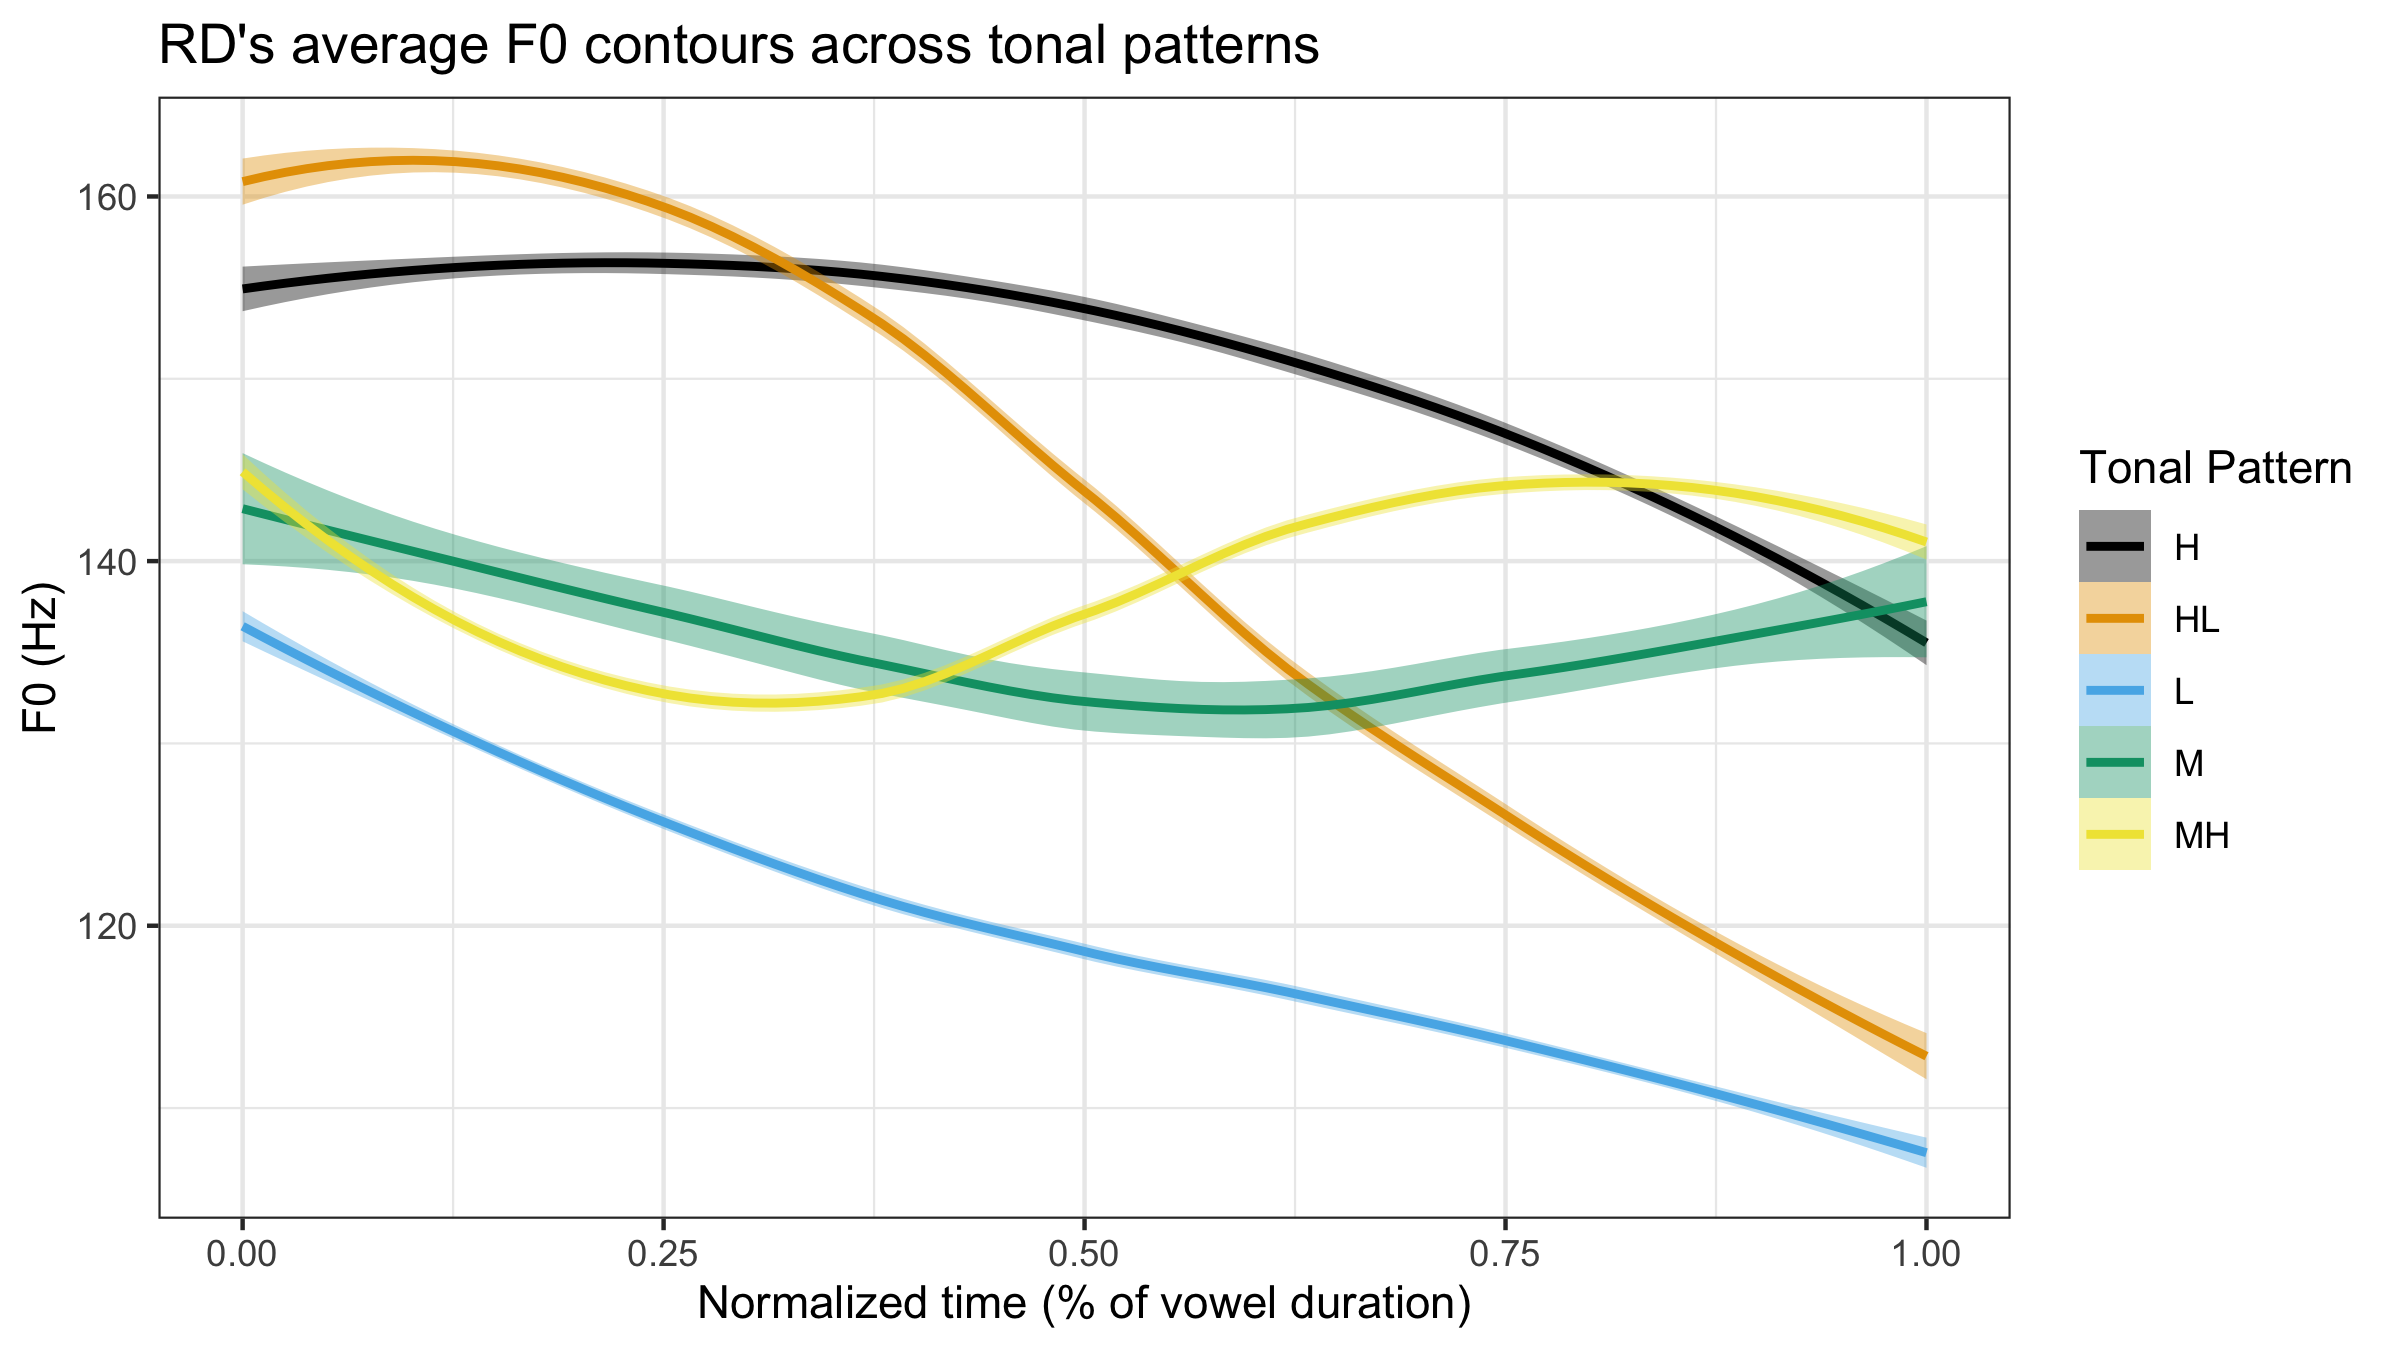
\includegraphics[width=0.9\textwidth]{../JoinTonePlot.png}
% 	\label{fig:LAMNetwork}
% 	\caption{Tonal contrasts for FSR and RD normalized for f0 and time.}
% \end{figure}

%------------------------------------
\subsection{Interaction of Tone and Phonation} \label{sec:Interaction}
%------------------------------------

Most previous work on the interaction of tone has been focused on the languages of East and Southeast Asia 
\citep[e.g.,][]{masicaDefiningLinguisticArea1976,thurgoodVietnameseTonogenesisRevising2002,yipTone2002,enfieldArealLinguisticsMainland2005,michaudComplexTonesEast2012,brunelleTonePhonationSoutheast2016}. 
What has been found in these descriptions is that certain tones and phonations are codependent (i.e., only occur with each other). For example \citet{smalleyProblemsConsonantsTone1976} and \citet{ratliffMeaningfulToneStudy1992} both describe White Hmong's \textit{-g} tone as being a mid-low tone with breathy phonation and Mandarin's tone 3 is often associated with creaky phonation \citep{hockettPeipingPhonology1947}. \citet{brunelleTonePerceptionNorthern2009} found that creaky phonaiton plays an important role in the production of certain tones. Additionally, work on S'gaw Karen has found that two tones are only differentiated by the presence of some form of amodal phonation (Boehm p.c.). 

However, there has been some observations–especially in Mesoamerican–that tone and phonation can co-vary \citep[e.g,][]{silvermanLaryngealComplexityOtomanguean1997,garellekAcousticConsequencesPhonation2011}. This means that tone can independently occur with any phonation type. This has also been extensively described in multiple Zapotecan languages \citep[e.g.,][]{,avelinobecerraTopicsYalalagZapotec2004,avelinoAcousticElectroglottographicAnalyses2010, chavez-peonInteractionMetricalStructure2010, campbellZenzontepecChatinoAspect2011,villardPhonologyMorphologyZacatepec2015, lopeznicolasEstudiosFonologiaGramatica2016}

\citet{chavez-peonInteractionMetricalStructure2010} has a detailed description of the tone and phonation interactions in San Lucas Quiaviní Zapotec (SLQZ), a central valley variety of Zapotec. The distribution of tone and phonation is found in Table~\ref{tab:SLQZ} and repeated below as Table~\ref{tab:SLQZrepeat}.
\begin{table}[!ht]
	\centering
	\caption{SLQZ tone and phonation interactions \citep{chavez-peonInteractionMetricalStructure2010}.}
	\label{tab:SLQZrepeat}
	 \begin{tabular}{lcccc}
	  \lsptoprule
					  &	 \textbf{Modal}  & \textbf{Breathy} & \textbf{Creaky} & \textbf{Interrupted} \\
		  High	& ✔︎ & -- & ✔︎ & ✔︎ \\
		  Low & ✔︎ & ✔︎ & ✔︎ & ✔︎ \\
		  Falling & ✔︎ & ✔︎ & ✔︎ & ✔︎ \\
		  Rising & ✔︎ & -- & -- & -- \\
	  \lspbottomrule
	 \end{tabular}
\end{table}

We see that in SLQZ, that both low and falling tone have the full range of possible combinations. However, we see gaps in the high tone for breathy and rising tone can only occur with modal phonation. 

Based on elicitation data collected from 2020-2022, SLZ has a more expansive distribution of tone and phonation when compared to SLQZ but seems to be very similar to other Northern Zapotec varities \citep[e.g.,][]{avelinobecerraTopicsYalalagZapotec2004}. The distribution of SLZ tonal and phonation interactions are given in Table~\ref{tab:ToneVoiceQuality}. 
\begin{table}[!h]
	\caption{Distribution of tone and phonation in SLZ}
	\label{tab:ToneVoiceQuality}
	\centering

	\begin{tabular}{lcccc}
	\lsptoprule
		& \textbf{Modal} & \textbf{Breathy} & \textbf{Checked} & \textbf{Laryngealized} \\
	\hline
	H	& ✔ & -- & ✔ & ✔ \\
	M	& ✔ & ✔ & ✔ & ✔\\
	L	& ✔	& ✔ & ✔ & ✔\\
	HL	& ✔	& ✔ & ✔ & ✔\\
	MH	& ✔	& ✔ & -- & ✔ \\
	\lspbottomrule
	\end{tabular}
\end{table}

The striking observations that we find is that there are some gaps in where breathy is allowed to occur. This is also true for the checked phonation. 


%------------------------------------
\section{Acoustic investigation into the phonation} \label{sec:Acoustics}
%------------------------------------

\begin{itemize}
	\item Spectral measurements have been found to be very useful measure of phonation in a wide number of different languages [ADD REFERENCES FROM ESPOSITO]. 
	\item Most of these have been focused on H1-H2, however, relationships with H1 compared to higher harmonics have also been found to be useful. 
	\item Most previous studies have not used corrected or normalized measure but have been focused on a single vowel /a/ because it minimizes the effects of the F1.
	\begin{itemize}
		\item Using corrected values is a way to mitigate the effects of the formants on the vowels. 
	\end{itemize}
	\item Describe how acoustic measurements are taken using \citet{garellekPhoneticsVoice2019} as a basis for how the measurements are taken. 
	\begin{itemize}
		\item maybe use SoE as well?
		\item Additionally, describe the patterns that we expect to see. 
	\end{itemize}
	\item Following \citet{espositoVariationContrastivePhonation2010}, I use H1-H2 and H1-A3. 
	\item Additionally, CPP is a useful measurement for modal versus a modal phonation \citep{garellekPhoneticsWhiteHmong2021}.
	\item Figure out what which charts are useful. Might be useful to follow \citet{espositoVariationContrastivePhonation2010} in taking measurements from a certain portion of the vowels. 
\end{itemize}

\begin{figure}[!ht]
	\includegraphics[width=0.9\textwidth]{../h1h2_CheckedLaryngeal.png}
	\caption{FSR's H1-h2 values for checked and laryngealized.}
	\label{fig:FSRh1h2checked} 
\end{figure}


\begin{figure}[!ht]
	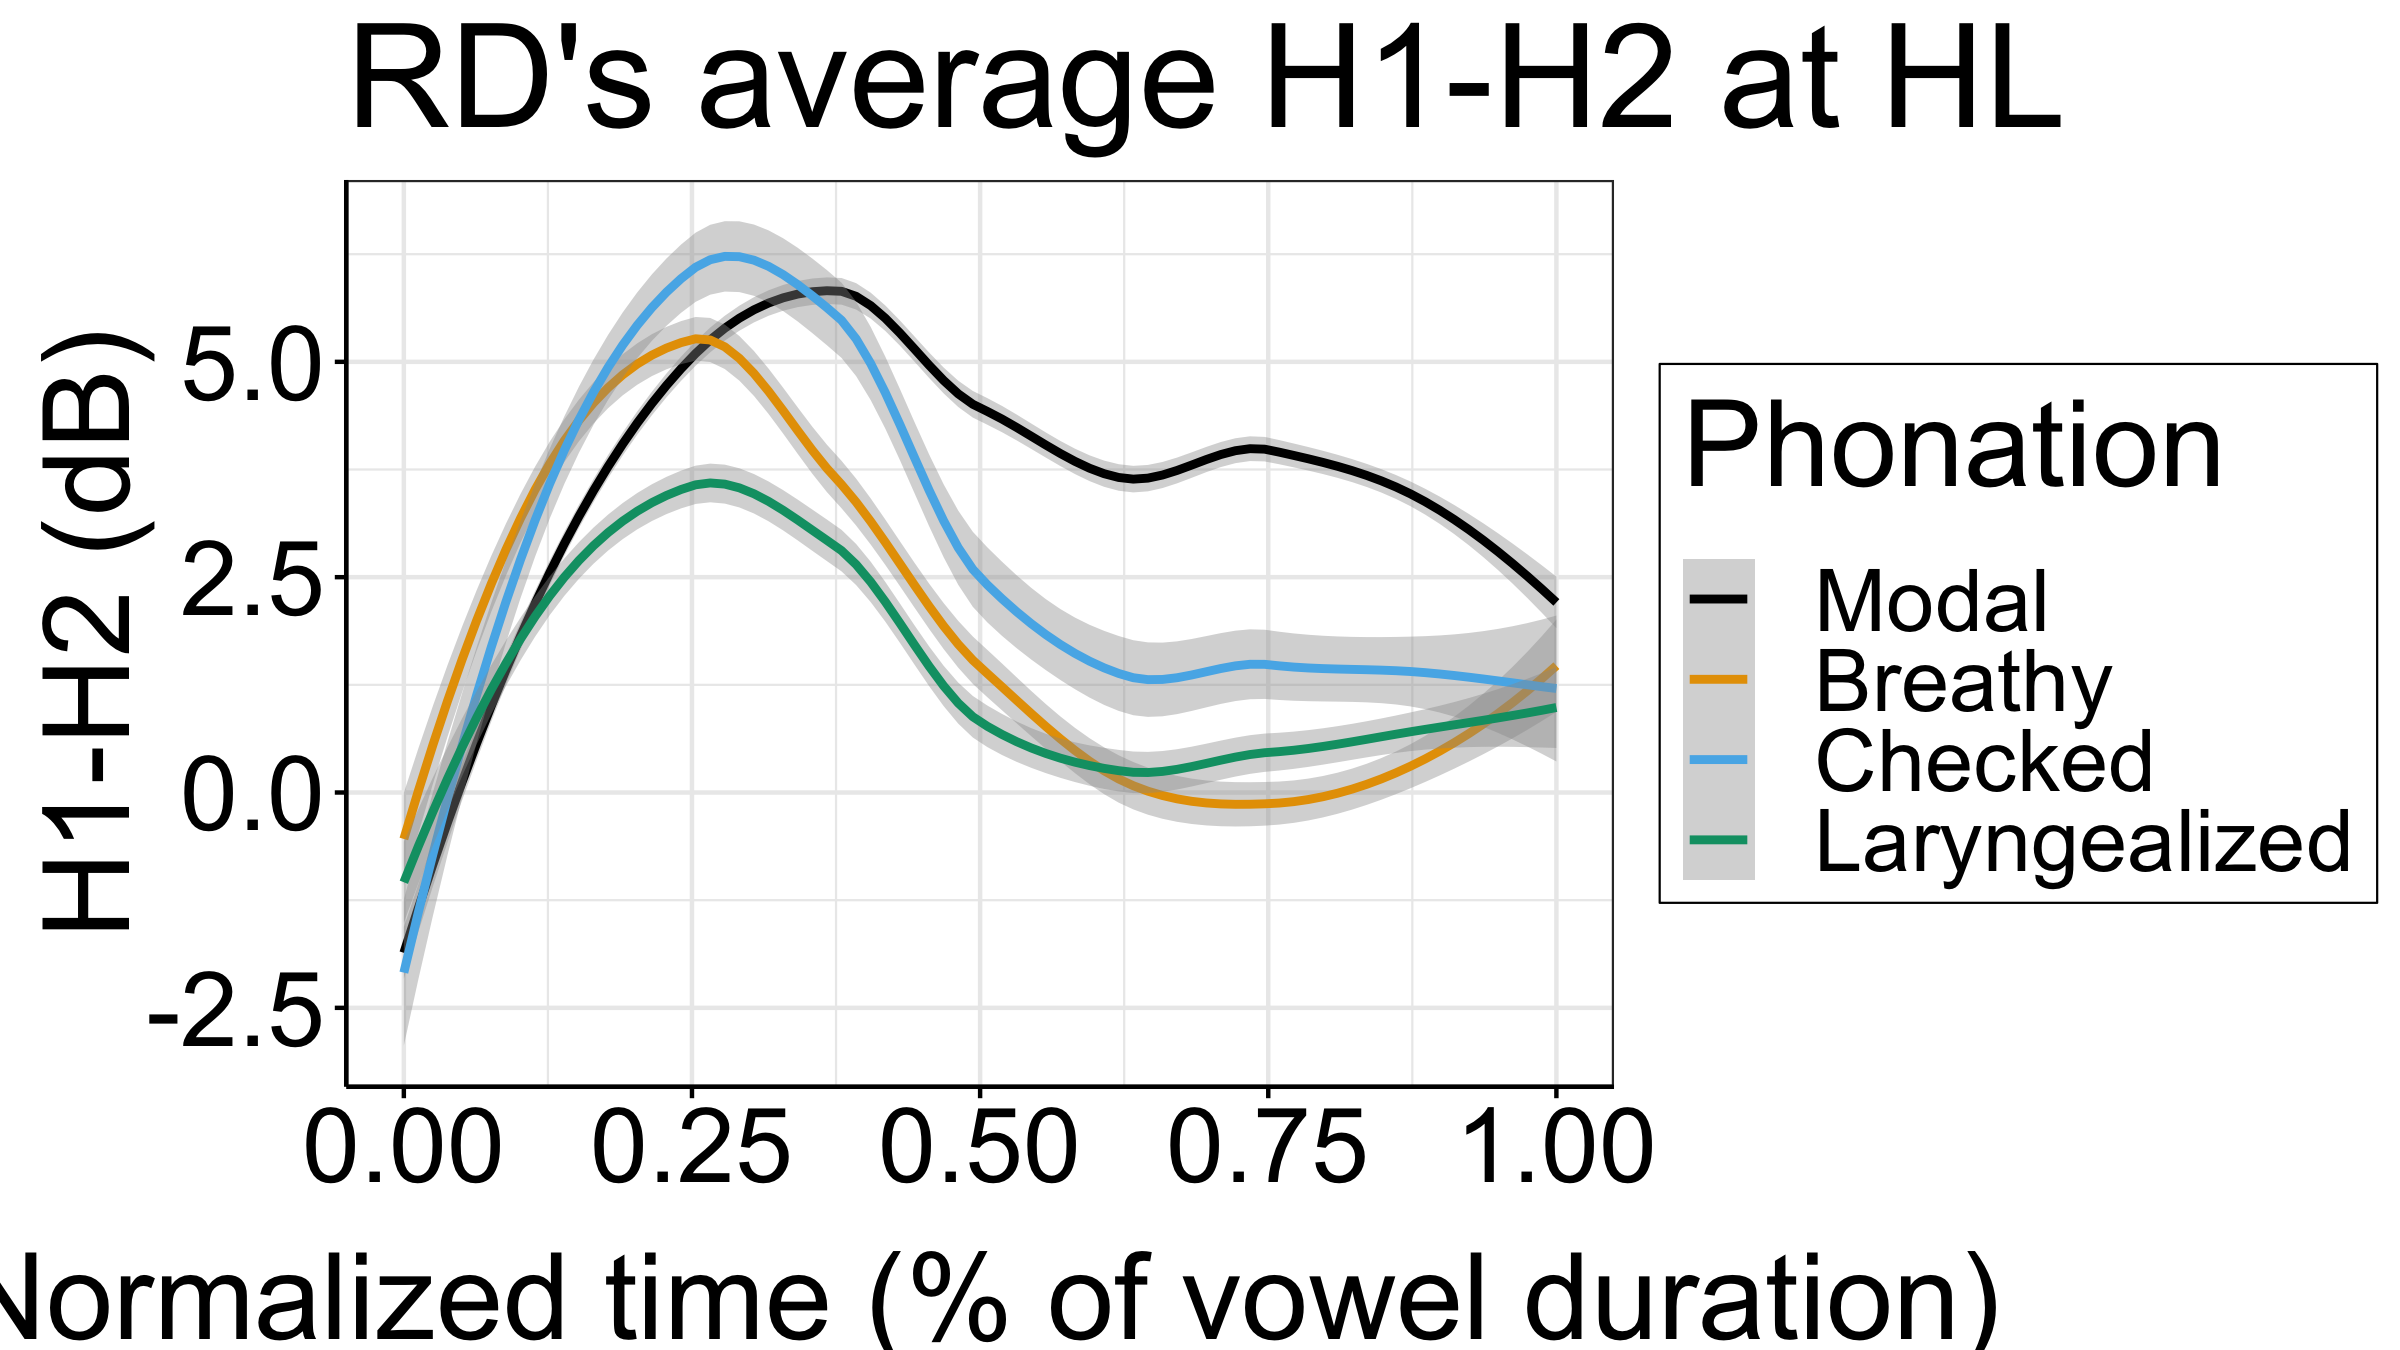
\includegraphics[width=0.9\textwidth]{../RDh1h2_line_HL.png}
	\caption{RD's H1-H2 values in HL toned syllables.}
	\label{fig:RDh1h2} 
\end{figure}


\begin{figure}[!ht]
	\includegraphics[width=0.9\textwidth]{../RDH1A3_HL.png}
	\caption{RD's total H1-A3 values in HL toned syllables. }
	\label{fig:RDh1a3} 
\end{figure}

	
\begin{figure}[!ht]
	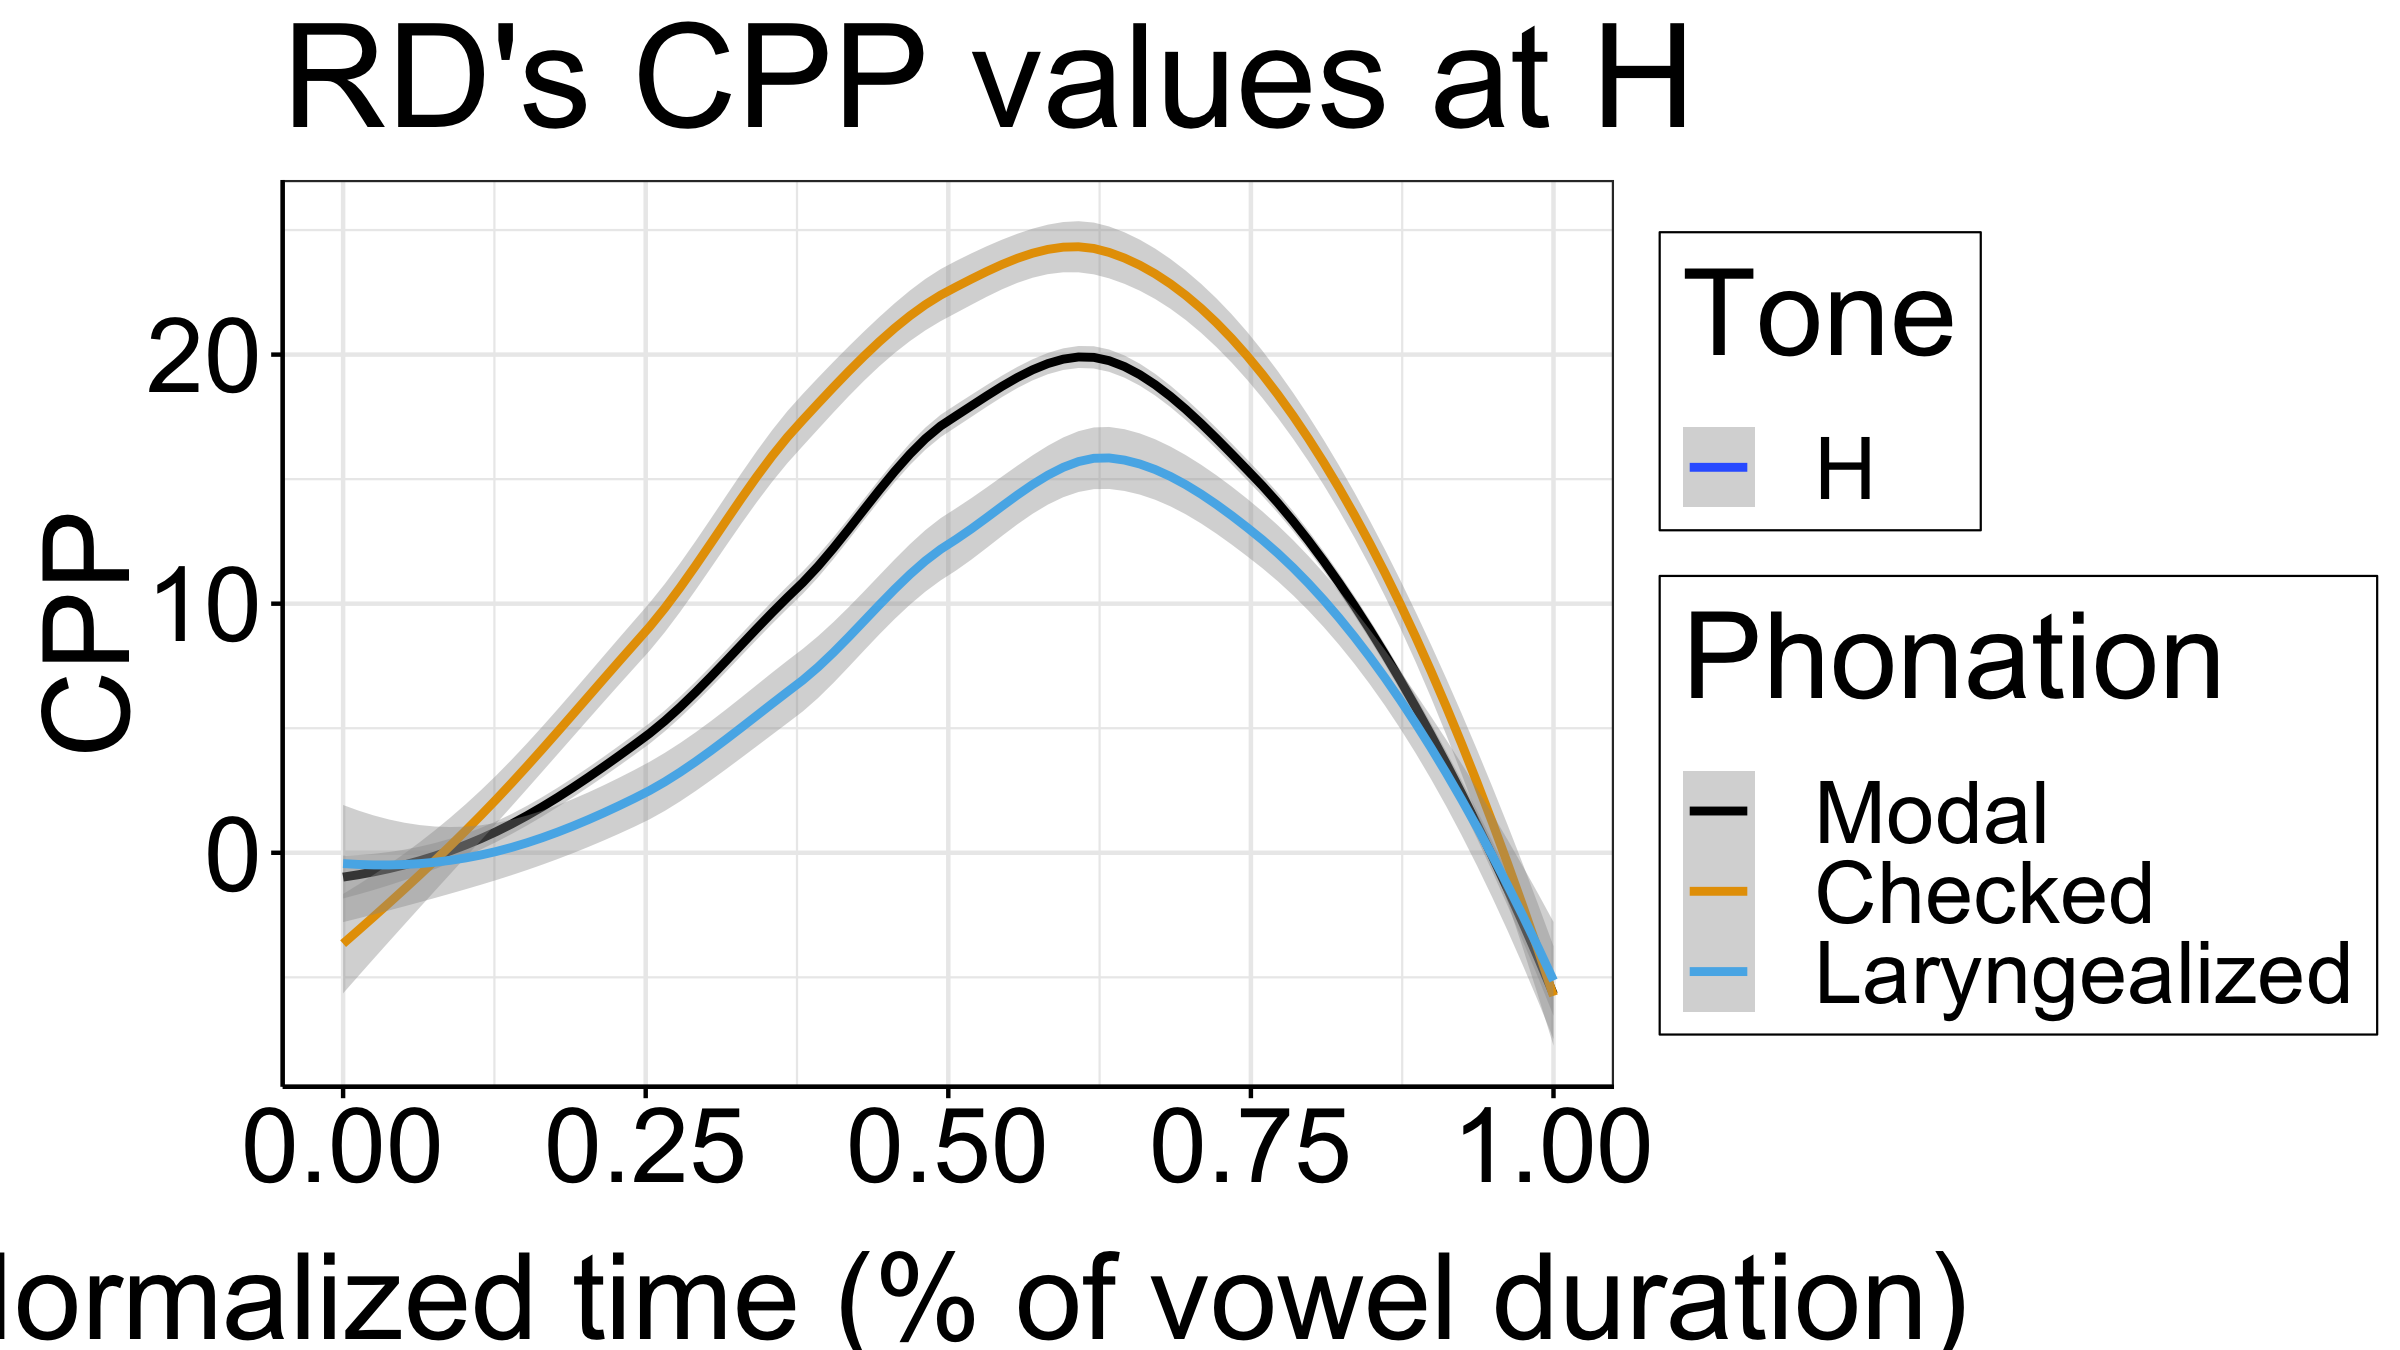
\includegraphics[width=0.9\textwidth]{../RDCPP_lineL.png}
	\caption{RD's CPP values.}
	\label{fig:RDCPP} 
\end{figure}	

\begin{itemize}
	\item Might be useful to validate h1-h2 and h1-a3 measurements as useful diagnostics. 
	\item What do the measurements show me?
	\begin{itemize}
		\item FSR shows a timing difference between checked and rearticulated in h1-h2.
		\item RD shows the differences we expect to see in h1-a3 but not 
	\end{itemize}
\end{itemize}

%------------------------------------
\section{Challenges to theories} \label{sec:Challenges}
%------------------------------------

\begin{itemize}
	\item How does this support or detract from \posscitet{silvermanLaryngealComplexityOtomanguean1997} claims?
	\begin{itemize}
		\item Do we see the gestural timing that \citet{silvermanLaryngealComplexityOtomanguean1997} claims to exist?
	\end{itemize}
	\item Issues with breathy not present with H. 
	\item Additionally there is this question about why we are seeing laryngealized vowels in H tone
	\begin{itemize}
		\item Could \posscitet{eslingVoiceQualityLaryngeal2019} model of interactions be used to explain what we are seeing?
	\end{itemize}
\end{itemize}




%------------------------------------
\section{Esposito 2010} \label{sec:Esposito}
%------------------------------------

\begin{itemize}
	\item Esposito investigates variation in Santa Ana del Valle Zapotec for variation due to gender, F0 and prosodic position.
	\item Results were inconclusive as to whether or not gender was creakier or breathier though the acoustic measurements (H1-H2 and H1-A3) suggest that there is a difference in \textsc{production}. 
	\item Strong effects of F0 were observed
	\item The phonation contrasts were present in all positions but were not always well-defined. 
	\item There has been a wide number of studies that have observed phonation differences based on gender, F0, and position. For example females are often described as being breathier than males (though this was not true all the time) and prosodic position produced different phonations. Additionally, all of these cases involve allophonic or suprasegmental phonation (i.e., non-phonemic)
	\item Very little work has investigated languages with phonemic phonation contrasts
	\item Jalapa Mazatec and San Lucas Quiaviní Zapotec are some of the few that have seen some study.
	\item In those studies females were breathier than the male speaker. 
	\item SADVZ is an ideal language to study the variation in phonation because it has relatively free word order and the contrastive phonation that exists. 
	\item Spectral measurements have been found to be very useful measure of phonation in a wide number of different languages. 
	\item Most of these have been focused on H1-H2, however, relationships with H1 compared to higher harmonics have also been found to be useful. 
	\item Most previous studies have not used corrected or normalized measure but have been focused on a single vowel /a/ because it minimizes the effects of the F1
	\item Esposito focuses on H1-H2 (open quotient) and H1-A3 (speed of vocal fold closure) based on a pilot study she ran in 2003. 
	\item Vowel measurements were made by splitting the vowel into four equal parts and h1-h2 and h1-h3 measurements were made in the last quarter of each vowel. 
	\item H1-A3 and H1*-A3* were effective in distinguishing the different phonation types in males. The difference between corrected and uncorrected were not significant. 
	\item H1-H2 was effective for females speakers. 
	\item The fact that h1-h2 was effective for females and h1-a3 for males suggests that they are using different laryngeal settings. Female speakers are making more use of open-quotient whereas male speakers are using the speed of vocal fold closure to distinguish the different phonation types. 
	\item When looking at whether or not there is an effect for prosodic position it was observed that F0 had more of an effect than position. 
	\item What was found was that all three contrasts were maintained but differed in how clearly they are produced. 
\end{itemize}

%------------------------------------
\section{DiCanio 2012} \label{sec:DiCanio}
%------------------------------------

\begin{itemize}
	\item \citeauthor{dicanioCoarticulationToneGlottal2012} is concerned with exploring the effects that tone and glottal consonants have on each other.
	
	\item Much of the earlier work on coarticulation claimed that the processes of the interaction of tone and phonation/glottal consonants revealed something universal or a set of constraints that applied to all languages.

	\item More recent work actually argues against this notion specifically that there aren’t language-wide or universality but instead is based on language-specific patterns.
	
	\item One of these areas has to do with the phasing or co-articulation discussion.
	
	\item One area that has received substantially less discussion is on the realm of tone and phonation type contrasts.
	
	\item This study serves two main purposes: (i) expand the emperical basis for the analysis of tone-segment coarticulation and (ii) test how changes in relative timing of glottal consonants affect F0 on adjacent vowels.
	
	\item One main question I have is that these contrasts that DiCanio is describing seem to be almost more akin to phonation contrasts instead of segmental changes. However, he does seem to have a good amount of information from his dissertation which suggests that these are segmental instead of qualities of the vowel \citep{dicanioPhoneticsPhonologySan2008}.
	
	\item There is some discussion about \citet{silvermanLaryngealComplexityOtomanguean1997} where glottal consonants are abruptly phased relative to the vowels.
	
	\item According to Silverman there needs to be abrupt phasing so listeners can distinguish the tone and the glottal contrast.
	
	\item Trique does a wonderful job to at allowing us to test this claim that there is abrupt phasing. Specifically this paper investigates whether the amount of coarticulatory overlap between glottals and vowels effect the F0 perturbation.
	
	\item Trique has prominence and is reflected by a large distribution of contrasts in the final-syllables of words. But these contrasts are neutralized in non-final syllables. Phonetically realized by increased duration
	
	\item Spectral tilt was used to measure the magnitude of glottal tension or spreading. H1-H2 is a useful diagnostic for differentiating breathy, modal, and tense/creaky phonation. Additionally, H1-A3 is useful for breathy vs. non-breathy.
	
	\item Results were z-transformed and then a linear mixed effects model was run with speaker as random.
	
	\item Breathy phonation is described as higher h1-h2 values and lower H1-H2 values with lower F0. Lower F0 is associated with breathy voice.
\end{itemize}

%------------------------------------
\section{Holmberg, et al. 1995} \label{sec:Holmberg}
%------------------------------------

\begin{itemize}
	\item \citet{holmbergComparisonsAerodynamicElectroglottographic1995} are interested in comparing different acoustic measuring systems. 
	\item Specifically, they were interested in seeing how aerodynamic, EGG, and spectral measures differed in capturing aspect of female voices. 
	\item They found the following seven things:
	\begin{enumerate}
		\item Significant differences in parameter values between /pTe/ and /a/ were related to significant differences in the sound pressure level (SPL).
		\item An ``adduction quotient," measured from the glottal waveform at a 30\% criterion, was sensitive enough to differentiate between waveforms reflecting abrupt versus gradual vocal fold closing movements. 
		\item DC flow showed weak or nonsignificant relationships with acoustic measures. 
		\item The spectral content in the third formant (F3) in comfortable loudness typically consisted of a mix of noise and harmonic energy. In loud voice, the F3 spectral content typically consisted of harmonic energy. 
		\item Significant differences were found in all measures between tokens with F3 harmonic energy and tokens with F3 noise, independent of loudness condition. 
		\item Strong relationships between flow- and EGG-adduction quotients suggested that these signals can be used to complement each other.
		\item The amplitude difference between spectral peaks of the first and third formant (F1 -F3) was found to add information about abruptness of airflow decrease (flow declination) that may be lost in the glottal waveform signal due to low-pass filtering.
	\end{enumerate}
	\item Even though EGG data was useful it was also extremely limited in nature. 
	\item They found that if the larynx was to small, the neck was to fat, or there was a lot of gross laryngeal movement that the EGG data was inconclusive. 
	\item EGG is best for determining the adduction quotient (closed time/T). 
\end{itemize}

%------------------------------------
\section{Conclusion} \label{sec:Conclusion}
%------------------------------------

%------------------------------------
%BIBLIOGRAPHY
%------------------------------------

%\singlespacing
% \nocite{*}
\printbibliography[heading=bibintoc]

\end{document} 